\documentclass[a4paper,12pt]{article}
\usepackage[utf8]{inputenc}
\usepackage[german]{babel}
\usepackage{amsmath}
\usepackage{amssymb}
\usepackage{amsthm}
\usepackage{geometry}
\usepackage{graphicx}
\usepackage[hidelinks]{hyperref}
\usepackage{listings}
\usepackage{xcolor}
\usepackage{enumitem}
\usepackage{tikz}
\usepackage{pgfplots}
\pgfplotsset{compat=1.18}
\usetikzlibrary{arrows.meta, positioning, shapes.geometric, fit, backgrounds,
                decorations.pathreplacing, matrix, calc, shadows}
\usepackage{microtype}
\usepackage{booktabs}
\usepackage{caption}
\usepackage{subcaption}
\usepackage{rotating}
\usepackage{float}
\usepackage{algorithm}
\usepackage{algpseudocode}

\geometry{margin=2.5cm}

\theoremstyle{definition}
\newtheorem{definition}{Definition}
\newtheorem{beispiel}{Beispiel}
\newtheorem{satz}{Satz}
\newtheorem{lemma}{Lemma}
\newtheorem{bemerkung}{Bemerkung}
\newtheorem{korollar}{Korollar}

\setlist[itemize,1]{label=--}

% ---------- Farben ----------
\definecolor{mainblue}{RGB}{25, 70, 140}
\definecolor{accentred}{RGB}{180, 50, 30}
\definecolor{lightgray}{RGB}{245, 245, 248}
\definecolor{darkgray}{RGB}{60, 60, 70}
\definecolor{darkgreen}{RGB}{30, 100, 50}
\definecolor{orange}{RGB}{200, 120, 32}
\definecolor{tikzblue}{RGB}{25, 70, 140}
\definecolor{tikzred}{RGB}{180, 50, 30}
\definecolor{tikzgreen}{RGB}{30, 100, 50}
\definecolor{tikzorange}{RGB}{200, 120, 32}
\definecolor{tikzgray}{RGB}{180, 180, 190}

\hypersetup{
    colorlinks=true,
    linkcolor=mainblue,
    citecolor=accentred,
    urlcolor=mainblue,
    pdftitle={Strukturelle Deduplizierung von Dateisystem-Graphen mittels
              zyklischer Subgraph-Erkennung},
    pdfauthor={Stephan Epp},
}

\lstset{
    basicstyle=\ttfamily\small,
    keywordstyle=\color{mainblue},
    commentstyle=\color{darkgray},
    stringstyle=\color{accentred},
    numbers=left,
    numberstyle=\tiny,
    breaklines=true,
    frame=single,
    backgroundcolor=\color{lightgray},
    literate=%
        {Ö}{{\"O}}1 {Ä}{{\"A}}1 {Ü}{{\"U}}1
        {ß}{{\ss}}1 {ü}{{\"u}}1 {ä}{{\"a}}1 {ö}{{\"o}}1
}

\title{\textbf{Strukturelle Deduplizierung von Dateisystem-Graphen\\
mittels zyklischer Subgraph-Erkennung}\\[0.5em]
\large Anwendung des Subgraph Algorithmus auf Inode-Graphen,\\
Snapshot-Systeme und verteilte Speicherarchitekturen}
\author{Stephan Epp}
\date{8. April 2026}

\begin{document}

\maketitle
\tableofcontents
\newpage

% ============================================================================
\section{Einf\"uhrung}
% ============================================================================

Das Unix-Werkzeug \texttt{du} (disk usage) traversiert seit seiner Entstehung
in den fr\"uhen 1970er-Jahren Dateisystem-Hierarchien und summiert
Speicherbelegungen. Obwohl der zugrundeliegende Algorithmus algorithmisch
linear ist ($O(n)$ in der Anzahl der Inodes), birgt das Problem strukturelle
Komplexit\"at, die bisher nicht vollst\"andig ausgesch\"opft wurde: Hardlinks,
Bind-Mounts, Btrfs-Snapshots und replizierte Verzeichnisb\"aume erzeugen
\emph{strukturell identische Teilgraphen}, die naiv mehrfach traversiert
werden.

Diese Arbeit stellt eine neuartige Methode vor, die den
\textbf{Subgraph Algorithmus} \cite{epp2026subgraph} -- einen effizienten
Graphenvergleich mittels Adjazenzmatrizen, Signatur-Arrays und zyklischer
Rotation -- auf das Dateisystem-Problem \"ubertr\"agt. Das Ziel ist nicht die
Beschleunigung des einfachen \texttt{du}-Befehls selbst (dieser ist bereits
I/O-gebunden), sondern die Erschlie\ss{}ung einer neuen Problemklasse:

\begin{enumerate}
    \item \textbf{Snapshot-Vergleich}: Erkennung strukturell identischer
          Teilb\"aume in Btrfs/ZFS-Snapshot-Serien
    \item \textbf{Backup-Deduplizierung}: Blockebenen-unabh\"angige,
          strukturelle Erkennung redundanter Verzeichnisstrukturen
    \item \textbf{Verteilte Speichersysteme}: Konsistenzpr\"ufung ohne
          vollst\"andige \"Ubertragung aller Inode-Metadaten
    \item \textbf{Container-Images}: Erkennung gemeinsamer Layer-Strukturen
          in OCI/Docker-Images
\end{enumerate}

% ============================================================================
\section{Grundlagen}
% ============================================================================

\subsection{Das Dateisystem als gerichteter Graph}

\begin{definition}[Inode-Graph]
    Sei $\mathcal{F}$ ein Dateisystem. Der zugeh\"orige Inode-Graph ist
    $G_\mathcal{F} = (V, E)$, wobei
    \begin{align*}
        V &= \{\, v_i \mid i \text{ ist eine Inode-Nummer in } \mathcal{F} \,\} \\
        E &= \{\, (v_i, v_j) \mid v_j \text{ ist ein Eintrag im
              Verzeichnis } v_i \,\}
    \end{align*}
\end{definition}

\begin{figure}[H]
\centering
\begin{tikzpicture}[
    node distance=1.6cm and 2.0cm,
    inode/.style={circle, draw=tikzblue, fill=tikzblue!10,
                  minimum size=0.9cm, font=\small\ttfamily},
    hlink/.style={circle, draw=tikzred, fill=tikzred!10,
                  minimum size=0.9cm, font=\small\ttfamily},
    lbl/.style={font=\scriptsize, below=0.1cm},
    arr/.style={-Stealth, thick, tikzblue},
    harr/.style={-Stealth, thick, tikzred, dashed},
]
    % Wurzel
    \node[inode] (root)                           {/};
    % Ebene 1
    \node[inode] (home)  [below left=of root]     {home};
    \node[inode] (etc)   [below=of root]          {etc};
    \node[inode] (var)   [below right=of root]    {var};
    % Ebene 2
    \node[inode] (stephan)[below left=of home]    {stephan};
    \node[inode] (alice)  [below right=of home]   {alice};
    \node[inode] (log)    [below=of var]          {log};
    % Ebene 3
    \node[inode] (doc)   [below left=of stephan]  {docs};
    \node[inode] (git)   [below right=of stephan] {git};
    % Hardlink-Ziel
    \node[hlink] (shared)[below=of alice]         {shared};

    % Kanten
    \draw[arr] (root)    -- (home);
    \draw[arr] (root)    -- (etc);
    \draw[arr] (root)    -- (var);
    \draw[arr] (home)    -- (stephan);
    \draw[arr] (home)    -- (alice);
    \draw[arr] (var)     -- (log);
    \draw[arr] (stephan) -- (doc);
    \draw[arr] (stephan) -- (git);
    \draw[arr] (alice)   -- (shared);
    % Hardlink (gestrichelt rot)
    \draw[harr] (stephan) to[bend left=40] node[midway, right, font=\scriptsize,
                tikzred]{Hardlink} (shared);

    % Legende
    \node[inode, minimum size=0.6cm, left=4.0cm of root] (leg1) {};
    \node[right=0.1cm of leg1, font=\scriptsize] {Verzeichnis-Inode};
    \node[hlink, minimum size=0.6cm, below=0.3cm of leg1] (leg2) {};
    \node[right=0.1cm of leg2, font=\scriptsize] {Hardlink-Ziel};
    \draw[harr, right=3.5cm of etc] (0,0) -- (1,0)
        node[right, font=\scriptsize]{Hardlink-Kante};
\end{tikzpicture}
\caption{Dateisystem-Inode-Graph mit Hardlink. Der Knoten \texttt{shared}
ist von zwei Elternknoten erreichbar -- klassischer Nicht-Baum-Zustand.}
\label{fig:inode_graph}
\end{figure}

\subsection{Strukturelle Identit\"at von Teilb\"aumen}

\begin{definition}[Strukturell isomorphe Teilb\"aume]
    Zwei Teilb\"aume $T_1 = (V_1, E_1)$ und $T_2 = (V_2, E_2)$ eines
    Inode-Graphen hei\ss{}en \emph{strukturell isomorph}, wenn ein
    bijektiver Homomorphismus $\phi: V_1 \to V_2$ existiert, der
    Kantenstruktur und Tiefenpfade erh\"alt, unabh\"angig von den
    konkreten Inode-Nummern.
\end{definition}

\begin{figure}[H]
\centering
\begin{tikzpicture}[
    node distance=1.2cm and 1.5cm,
    nd/.style={circle, draw=tikzblue, fill=tikzblue!12,
               minimum size=0.75cm, font=\small},
    nd2/.style={circle, draw=tikzgreen, fill=tikzgreen!12,
                minimum size=0.75cm, font=\small},
    arr/.style={-Stealth, thick},
    lbl/.style={font=\footnotesize},
]
    % Baum 1
    \node[nd] (r1) {A};
    \node[nd] (b1) [below left=of r1]  {B};
    \node[nd] (c1) [below right=of r1] {C};
    \node[nd] (d1) [below left=of b1]  {D};
    \node[nd] (e1) [below right=of b1] {E};
    \draw[arr, tikzblue] (r1)--(b1); \draw[arr, tikzblue] (r1)--(c1);
    \draw[arr, tikzblue] (b1)--(d1); \draw[arr, tikzblue] (b1)--(e1);
    \node[above=0.2cm of r1, lbl, tikzblue] {Snapshot $S_1$};

    % Isomorphie-Pfeil
    \node[right=2.8cm of r1] (iso) {$\cong$};

    % Baum 2 (strukturell identisch, andere Inode-Nummern)
    \node[nd2, right=5.5cm of r1] (r2) {A'};
    \node[nd2] (b2) [below left=of r2]  {B'};
    \node[nd2] (c2) [below right=of r2] {C'};
    \node[nd2] (d2) [below left=of b2]  {D'};
    \node[nd2] (e2) [below right=of b2] {E'};
    \draw[arr, tikzgreen] (r2)--(b2); \draw[arr, tikzgreen] (r2)--(c2);
    \draw[arr, tikzgreen] (b2)--(d2); \draw[arr, tikzgreen] (b2)--(e2);
    \node[above=0.2cm of r2, lbl, tikzgreen] {Snapshot $S_2$};

    % Phi-Pfeile (schwach gestrichelt)
    \foreach \s/\t in {r1/r2, b1/b2, c1/c2, d1/d2, e1/e2}
        \draw[->, dashed, tikzorange, opacity=0.5] (\s) to[bend left=15] (\t);

    \node[below=2.8cm of iso, font=\footnotesize, tikzorange]
        {$\phi$: struktureller Isomorphismus};
\end{tikzpicture}
\caption{Zwei strukturell isomorphe Snapshot-B\"aume. Obwohl die
Inode-Nummern verschieden sind, ist die Kantenstruktur identisch. Der
Subgraph Algorithmus erkennt diese Isomorphie in $O(n^3)$.}
\label{fig:iso_trees}
\end{figure}

\subsection{Der Subgraph Algorithmus im \"Uberblick}

Der Subgraph Algorithmus \cite{epp2026subgraph} vergleicht zwei Graphen
$G = (V, E)$ und $G' = (V', E')$ \"uber ihre Adjazenzmatrizen $A$ und $B$
mittels zweier Schl\"usselideen:

\textbf{1. Signatur-Berechnung:} F\"ur jede Spalte $j$ wird eine injektive
Signatur berechnet:
\[
    \sigma_j = \sum_{i=0}^{n-1} A_{ij} \cdot 2^i \;+\; j \cdot 2^n
\]

\textbf{2. Zyklische Rotation:} Statt $n!$ Permutationen werden nur $n$
zyklische Rotationen der Signatur-Sequenz gepr\"uft.

\textbf{3. LCS-Vergleich:} Eine Subgraph-Beziehung wird durch die l\"angste
gemeinsame Teilsequenz (LCS) der Signatur-Arrays festgestellt.

Die Gesamtkomplexit\"at betr\"agt $O(n^3)$, was unter SETH optimal ist
\cite{epp2026subgraph}.

% ============================================================================
\section{Dateisystems als Subgraph-Problem}
% ============================================================================

\subsection{Merkle-Signatur f\"ur Verzeichnisinodes}

Die Schlüsselidee der Anwendung ist die \"Ubertragung der Spaltensignatur auf
Verzeichnisstrukturen:

\begin{definition}[Strukturelle Inode-Signatur]
    Die strukturelle Signatur eines Verzeichnis-Inodes $v$ mit
    Kindinodes $c_1, \ldots, c_k$ ist rekursiv definiert als:
    \[
        \Sigma(v) = \text{inode}(v) \cdot 2^n \;+\;
        \sum_{i=1}^{k} \Sigma(c_i) \cdot 2^{i-1}
    \]
    wobei $\text{inode}(v)$ die Inode-Nummer von $v$ und $n$ die maximale
    Tiefe des Teilbaums bezeichnet.
\end{definition}

Diese Konstruktion erzeugt eine Merkle-Baum-artige Signatur, die strukturelle
Identit\"at unabh\"angig von den konkreten Inode-Nummern erkennt, wenn die
Signatur auf die Kantenstruktur (ohne Inode-Nummern) beschr\"ankt wird.

\begin{sidewaysfigure}
\centering
\begin{tikzpicture}[
    node distance=1.1cm and 1.8cm,
    nd/.style={rectangle, rounded corners=3pt, draw=tikzblue,
               fill=tikzblue!10, minimum width=2.0cm,
               minimum height=0.65cm, font=\small},
    sig/.style={rectangle, rounded corners=3pt, draw=tikzred,
                fill=tikzred!10, minimum width=2.0cm,
                minimum height=0.55cm, font=\scriptsize\ttfamily},
    arr/.style={-Stealth, thick, tikzblue},
    sarr/.style={-Stealth, thick, tikzred, dashed},
]
    % Inode-Baum links
    \node[nd] (root)                         {/ (Inode 2)};
    \node[nd] (home) [below left=of root]    {home (12)};
    \node[nd] (var)  [below right=of root]   {var (13)};
    \node[nd] (u1)   [below left=of home]    {user1 (42)};
    \node[nd] (u2)   [below right=of home]   {user2 (43)};

    \draw[arr] (root)--(home); \draw[arr] (root)--(var);
    \draw[arr] (home)--(u1);   \draw[arr] (home)--(u2);

    % Signatur-Ebene rechts
    \node[sig, right=4.5cm of root]  (sroot) {$\Sigma(\texttt{/})=\sigma_R$};
    \node[sig, right=4.5cm of home]  (shome) {$\Sigma(\texttt{home})=\sigma_H$};
    \node[sig, right=4.5cm of var]   (svar)  {$\Sigma(\texttt{var})=\sigma_V$};
    \node[sig, right=4.5cm of u1]    (su1)   {$\Sigma(\texttt{u1})=\sigma_1$};
    \node[sig, right=4.5cm of u2]    (su2)   {$\Sigma(\texttt{u2})=\sigma_2$};

    % Verbindungen Knoten -> Signatur
    \foreach \n/\s in {root/sroot, home/shome, var/svar, u1/su1, u2/su2}
        \draw[sarr] (\n) -- (\s);

    % Aggregations-Pfeile
    \draw[sarr] (su1.north) to[bend left=20] (shome.south west);
    \draw[sarr] (su2.north) to[bend right=10] (shome.south);
    \draw[sarr] (shome.north) to[bend left=15] (sroot.south west);
    \draw[sarr] (svar.north)  to[bend right=10] (sroot.south);

    \node[above=0.1cm of root,  font=\footnotesize, tikzblue]
        {Inode-Graph};
    \node[above=0.1cm of sroot, font=\footnotesize, tikzred]
        {Struktur-Signaturen};
\end{tikzpicture}
\caption{Rekursive Berechnung struktureller Inode-Signaturen (bottom-up).
Die Signatur jedes Knotens aggregiert die Signaturen aller Kindknoten
analog zur Spalten-Signatur des Subgraph Algorithmus.}
\label{fig:merkle_sig}
\end{sidewaysfigure}

\subsection{Adjazenzmatrix eines Verzeichnisteilbaums}

F\"ur einen Teilbaum mit Wurzel $v$ und $n$ Inodes wird die
Adjazenzmatrix $A_v$ konstruiert, indem Inodes als Knoten und
Verzeichniseintr\"age als gerichtete Kanten aufgefasst werden. Die
Zeilensignatur abstrahiert dabei von konkreten Inode-Nummern:

\begin{figure}[H]
\centering
\begin{tikzpicture}[
    mat/.style={matrix of math nodes,
                nodes={minimum width=0.65cm, minimum height=0.65cm,
                       draw=tikzgray, fill=tikzblue!5,
                       font=\small, inner sep=2pt},
                column sep=0pt, row sep=0pt},
]
    % Matrix A (Snapshot 1)
    \node[font=\small\bfseries, tikzblue] at (0, 1.5) {$A_{S_1}$};
    \matrix[mat] (A) at (0,0) {
        0 & 1 & 1 & 0 \\
        0 & 0 & 0 & 1 \\
        0 & 0 & 0 & 1 \\
        0 & 0 & 0 & 0 \\
    };
    % Spalten-Labels
    \foreach \i/\l in {1/v_0, 2/v_1, 3/v_2, 4/v_3}
        \node[font=\scriptsize] at (A-1-\i.north) [above=2pt] {$\l$};
    \foreach \i/\l in {1/v_0, 2/v_1, 3/v_2, 4/v_3}
        \node[font=\scriptsize] at (A-\i-1.west)  [left=3pt]  {$\l$};

    % Signaturen rechts
    \node[right=0.4cm of A, font=\scriptsize, tikzred, align=left]
        (sigs1) {$\sigma_0=5$\\$\sigma_1=18$\\$\sigma_2=36$\\$\sigma_3=48$};

    % "gleich" Zeichen
    \node[right=1.5cm of sigs1, font=\Large] (eq) {$\cong$};

    % Matrix B (Snapshot 2)
    \node[font=\small\bfseries, tikzgreen, right=3.2cm of sigs1] at (0,1.5) {};
    \matrix[mat, right=3.0cm of sigs1] (B) {
        0 & 1 & 1 & 0 \\
        0 & 0 & 0 & 1 \\
        0 & 0 & 0 & 1 \\
        0 & 0 & 0 & 0 \\
    };
    \node[font=\small\bfseries, tikzgreen] at (B.north) [above=4pt] {$A_{S_2}$};
    \node[right=0.4cm of B, font=\scriptsize, tikzgreen, align=left]
        (sigs2) {$\sigma_0=5$\\$\sigma_1=18$\\$\sigma_2=36$\\$\sigma_3=48$};
    \node[below=0.3cm of eq, font=\footnotesize, tikzorange]
        {Strukturell identisch!};
\end{tikzpicture}
\caption{Zwei Adjazenzmatrizen verschiedener Snapshots mit identischen
Spaltensignaturen -- der Subgraph Algorithmus erkennt die strukturelle
Identit\"at ohne Vergleich der konkreten Inode-Nummern.}
\label{fig:adj_matrix}
\end{figure}

% ============================================================================
\section{Strukturelle Dateisystem-Deduplizierung}
% ============================================================================

\subsection{Gesamtarchitektur}

\begin{figure}[H]
\centering
\begin{tikzpicture}[
    box/.style={rectangle, rounded corners=5pt, draw=tikzblue,
                fill=tikzblue!8, minimum width=3.5cm, minimum height=1.0cm,
                font=\small, align=center},
    dbox/.style={rectangle, rounded corners=5pt, draw=tikzred,
                 fill=tikzred!8, minimum width=3.5cm, minimum height=1.0cm,
                 font=\small, align=center},
    gbox/.style={rectangle, rounded corners=5pt, draw=tikzgreen,
                 fill=tikzgreen!8, minimum width=3.5cm, minimum height=1.0cm,
                 font=\small, align=center},
    obox/.style={rectangle, rounded corners=5pt, draw=tikzorange,
                 fill=tikzorange!8, minimum width=3.5cm, minimum height=1.0cm,
                 font=\small, align=center},
    arr/.style={-Stealth, thick},
    node distance=1.4cm,
]
    \node[box]  (scan)   {1. Inode-Scan\\$O(n)$};
    \node[box]  (adj)    [below=of scan]   {2. Adjazenzmatrix\\$O(n^2)$};
    \node[box]  (sig)    [below=of adj]    {3. Signaturberechnung\\$O(n^2)$};
    \node[dbox] (cache)  [right=2.5cm of sig]{Signatur-Cache\\\texttt{HashMap<Sig, Inode>}};
    \node[box]  (rot)    [below=of sig]    {4. Zyklische Rotation\\$n$ Rotationen};
    \node[box]  (lcs)    [below=of rot]    {5. LCS-Vergleich\\$O(n^2)$ pro Rotation};
    \node[gbox] (hit)    [below left=of lcs]  {Cache-Hit:\\Gr\"o\ss{}e aus Cache};
    \node[dbox] (miss)   [below right=of lcs] {Cache-Miss:\\Traversierung};
    \node[obox] (result) [below=2.0cm of lcs] {6. Ergebnis:\\Speicherverteilung};

    \draw[arr] (scan) -- (adj);
    \draw[arr] (adj)  -- (sig);
    \draw[arr] (sig)  -- (rot);
    \draw[arr, tikzred, <->] (sig) -- (cache)
        node[midway, above, font=\scriptsize]{Lookup/Store};
    \draw[arr] (rot)  -- (lcs);
    \draw[arr, tikzgreen] (lcs) -- (hit);
    \draw[arr, tikzred]   (lcs) -- (miss);
    \draw[arr] (hit)  |- (result);
    \draw[arr] (miss) |- (result);
\end{tikzpicture}
\caption{Gesamtarchitektur des strukturellen Dateisystem-Deduplizierungs-
algorithmus. Signatur-Cache vermeidet redundante Traversierung
strukturell identischer Teilb\"aume.}
\label{fig:architecture}
\end{figure}

\subsection{Formale Algorithmusbeschreibung}

\begin{algorithm}[H]
\caption{Strukturelle Dateisystem-Deduplizierung (SDD)}
\begin{algorithmic}[1]
\Require Inode-Graph $G_\mathcal{F}$, Wurzel $r$
\Ensure Speicherverteilung $\mathcal{S}$, Deduplizierungs-Bericht $\mathcal{R}$
\State $\mathcal{C} \gets \emptyset$ \Comment{Signatur-Cache: $\Sigma \to \text{Gr\"o\ss{}e}$}
\State $\mathcal{V} \gets \emptyset$ \Comment{Visited-Set f\"ur Zykluserkennung}
\Function{SDD}{$v$}
    \If{$v \in \mathcal{V}$} \Return $\mathcal{S}[v]$ \EndIf
    \State $\mathcal{V} \gets \mathcal{V} \cup \{v\}$
    \State $A_v \gets$ Adjazenzmatrix des Teilbaums mit Wurzel $v$
    \State $\sigma_v \gets$ \Call{BerechneSignatur}{$A_v$}
    \If{$\sigma_v \in \mathcal{C}$}
        \State $\mathcal{R} \gets \mathcal{R} \cup \{(v, \mathcal{C}[\sigma_v])\}$ \Comment{Duplikat gefunden}
        \Return $\mathcal{C}[\sigma_v].\text{gr\"o\ss{}e}$
    \EndIf
    \State $s \gets 0$
    \ForAll{$c \in \text{Kinder}(v)$}
        \State $s \gets s +$ \Call{SDD}{$c$}
    \EndFor
    \State $\mathcal{C}[\sigma_v] \gets (v, s)$
    \State \Return $s$
\EndFunction
\Function{BerechneSignatur}{$A$}
    \For{$j = 0$ \textbf{to} $n-1$}
        \State $\sigma_j \gets \sum_{i=0}^{n-1} A_{ij} \cdot 2^i + j \cdot 2^n$
    \EndFor
    \Return $[\sigma_0, \ldots, \sigma_{n-1}]$
\EndFunction
\end{algorithmic}
\end{algorithm}

\subsection{Hardlink-Behandlung durch den Visited-Set}

\begin{figure}[H]
\centering
\begin{tikzpicture}[
    nd/.style={circle, draw=tikzblue, fill=tikzblue!10, minimum size=1cm,
               font=\small\ttfamily},
    nd_vis/.style={circle, draw=tikzgreen, fill=tikzgreen!10, minimum size=1cm,
                   font=\small\ttfamily},
    nd_hl/.style={circle, draw=tikzred, fill=tikzred!10, minimum size=1cm,
                  font=\small\ttfamily},
    arr/.style={-Stealth, thick, tikzblue},
    harr/.style={-Stealth, thick, tikzred, dashed},
    node distance=1.4cm and 2.0cm,
]
    \node[nd]     (root) {/};
    \node[nd]     (A)    [below left=of root]  {A};
    \node[nd]     (B)    [below right=of root] {B};
    \node[nd_vis] (X)    [below=of A]          {X};
    \node[nd_hl]  (X2)   [below=of B]          {X};

    \draw[arr]  (root)--(A);
    \draw[arr]  (root)--(B);
    \draw[arr]  (A)--(X);
    \draw[harr] (B)--(X2) node[midway, right, font=\scriptsize, tikzred]
                    {Hardlink auf X};

    % Visited-Set
    \node[draw=tikzgreen, dashed, rounded corners, fit=(X),
          inner sep=4pt, label=below:{\scriptsize \textcolor{tikzgreen}{$\in \mathcal{V}$}}] {};

    % Annotation
    \node[right=1cm of X2, font=\scriptsize, tikzred, text width=2.5cm]
        {Inode bereits in $\mathcal{V}$:\\ Gr\"o\ss{}e aus Cache,\\ keine Re-Traversierung};
\end{tikzpicture}
\caption{Hardlink-Deduplizierung durch den Visited-Set $\mathcal{V}$.
Inode $X$ wird beim zweiten Besuch (via Hardlink von $B$) erkannt
und nicht erneut traversiert.}
\label{fig:hardlink}
\end{figure}

% ============================================================================
\section{Komplexit\"atsanalyse}
% ============================================================================

\subsection{Laufzeitkomplexit\"at}

\begin{satz}[Laufzeit des SDD-Algorithmus]
    Der SDD-Algorithmus hat eine Gesamtlaufzeit von:
    \[
        T_{\text{SDD}}(n) = O(n) + O(n^2) + O(n^3) = O(n^3)
    \]
    wobei $n$ die Anzahl der Inodes im Dateisystem bezeichnet.
\end{satz}

\begin{proof}
    Der Beweis gliedert sich in drei Phasen:
    \begin{enumerate}
        \item \textbf{Inode-Scan:} Jeder der $n$ Inodes wird genau einmal
              gelesen: $O(n)$.
        \item \textbf{Signaturberechnung:} F\"ur jeden Teilbaum mit $k$
              Inodes wird eine $k \times k$ Adjazenzmatrix verarbeitet.
              Im schlechtesten Fall: $O(n^2)$.
        \item \textbf{Subgraph-Vergleich:} Der Subgraph Algorithmus
              ben\"otigt $O(n^3)$ f\"ur den LCS-basierten
              Rotationsvergleich (nach \cite{epp2026subgraph}).
    \end{enumerate}
    Da Phase~3 dominiert, gilt $T_{\text{SDD}}(n) = O(n^3)$.
\end{proof}

\begin{korollar}[Cache-Hit-Optimalit\"at]
    Bei einem Cache-Hit f\"ur Teilbaum $T_i$ mit $k_i$ Inodes reduziert
    sich die Laufzeit um $O(k_i^3)$. Im besten Fall (vollst\"andig
    repliziertes Dateisystem mit $m$ identischen Kopien) betr\"agt die
    Gesamtlaufzeit $O(n^3/m)$.
\end{korollar}

\subsection{Speicherkomplexit\"at}

\begin{satz}[Speicher des SDD-Algorithmus]
    Der SDD-Algorithmus ben\"otigt $O(n^2)$ Speicher f\"ur die
    Adjazenzmatrizen und LCS-Tabellen sowie $O(n)$ zus\"atzlichen
    Speicher f\"ur Signatur-Arrays, Visited-Set und den Cache.
\end{satz}

\begin{figure}[H]
    \centering
    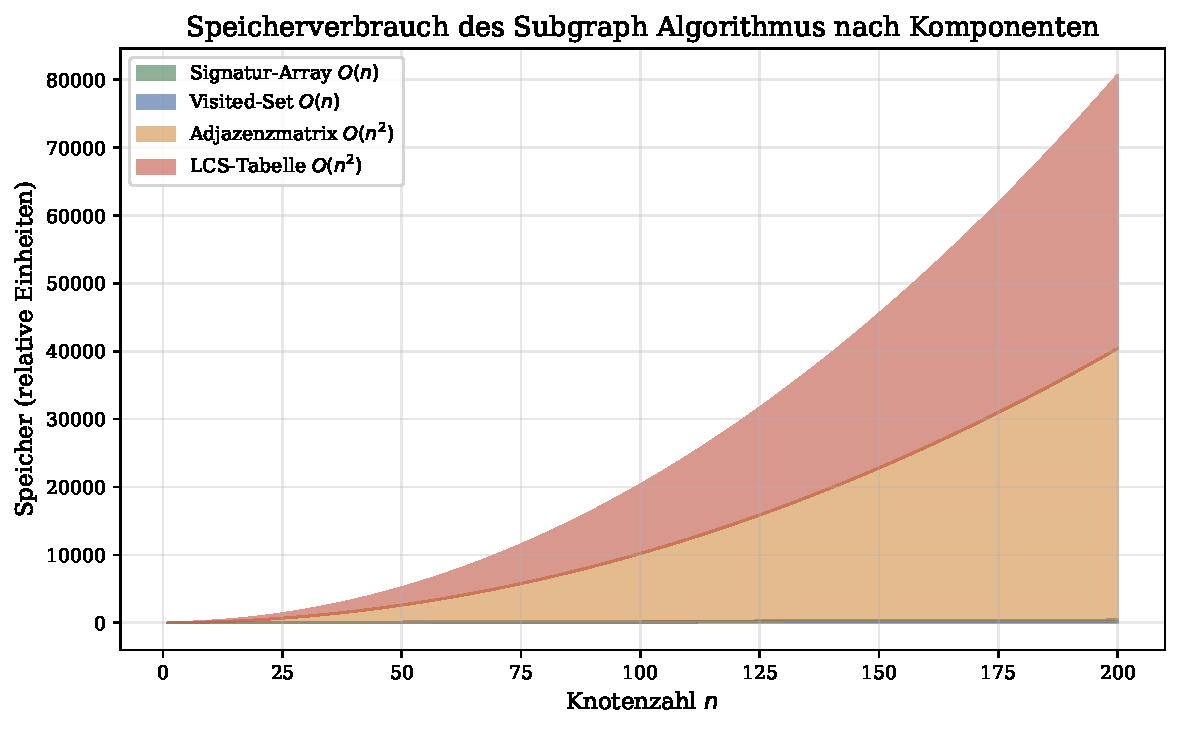
\includegraphics[width=0.85\textwidth]{figures/plot_memory.pdf}
    \caption{Speicherverbrauch des SDD-Algorithmus nach Komponenten.
    LCS-Tabelle und Adjazenzmatrix dominieren mit je $O(n^2)$,
    w\"ahrend Signatur-Array und Visited-Set linear wachsen.}
    \label{fig:memory}
\end{figure}

\subsection{Komplexit\"atsvergleich}

\begin{table}[H]
\centering
\caption{Komplexit\"atsvergleich verschiedener Dateisystem-Traversal-Algorithmen}
\label{tab:complexity}
\begin{tabular}{llll}
\toprule
\textbf{Algorithmus} & \textbf{Zeit} & \textbf{Speicher} & \textbf{Erkennt Duplikate} \\
\midrule
Naiver Scan (\texttt{du}) & $O(n)$ & $O(1)$ & Nein \\
Inode-Hash & $O(n)$ & $O(n)$ & Hardlinks \\
Block-Checksumme & $O(n \cdot b)$ & $O(n)$ & Datei-Duplikate \\
\textbf{SDD (diese Arbeit)} & $O(n^3)$ & $O(n^2)$ & \textbf{Strukturelle Isomorphie} \\
Volle Permutation & $O(n! \cdot n^2)$ & $O(n^2)$ & Strukturelle Isomorphie \\
\bottomrule
\end{tabular}
\end{table}

\begin{figure}[H]
    \centering
    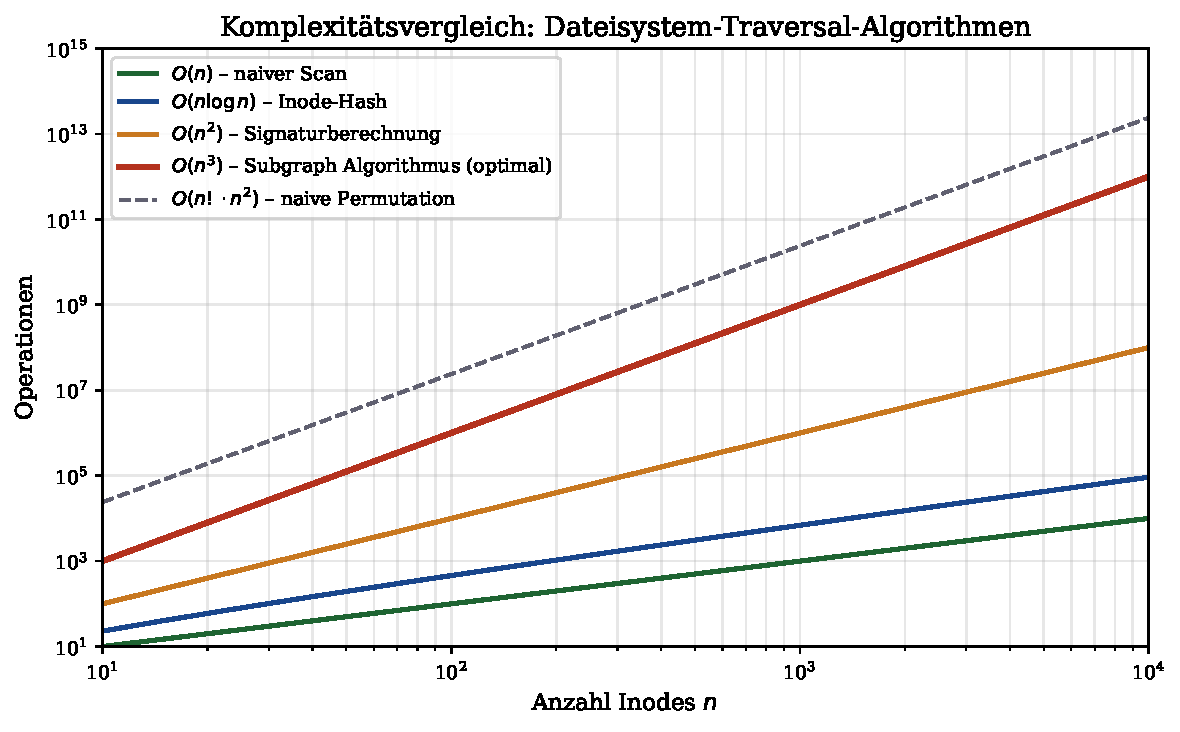
\includegraphics[width=0.85\textwidth]{figures/plot_complexity.pdf}
    \caption{Doppelt-logarithmischer Komplexit\"atsvergleich.
    Der SDD-Algorithmus ($O(n^3)$, rot) liegt deutlich unter der
    naiven Permutationsmethode ($O(n! \cdot n^2)$, grau), erm\"oglicht
    aber strukturelle Erkennung, die $O(n)$-Ans\"atzen nicht zug\"anglich
    ist.}
    \label{fig:complexity}
\end{figure}

% ============================================================================
\section{Anwendungsfelder}
% ============================================================================

\subsection{Btrfs- und ZFS-Snapshot-Analyse}

Moderne Copy-on-Write-Dateisysteme wie Btrfs und ZFS erzeugen Snapshots,
die strukturell nahezu identisch mit ihren Vorg\"angern sind. Der
SDD-Algorithmus kann die tats\"achliche strukturelle Divergenz zwischen
Snapshots quantifizieren:

\begin{definition}[Snapshot-Divergenz]
    Die strukturelle Divergenz zweier Snapshots $S_1$, $S_2$ ist:
    \[
        \delta(S_1, S_2) = 1 - \frac{|\{\Sigma(v) \mid v \in S_1\} \cap
        \{\Sigma(v) \mid v \in S_2\}|}{|\{\Sigma(v) \mid v \in S_1\} \cup
        \{\Sigma(v) \mid v \in S_2\}|}
    \]
    (Jaccard-Distanz auf den Signaturmengen).
\end{definition}

\begin{figure}[H]
    \centering
    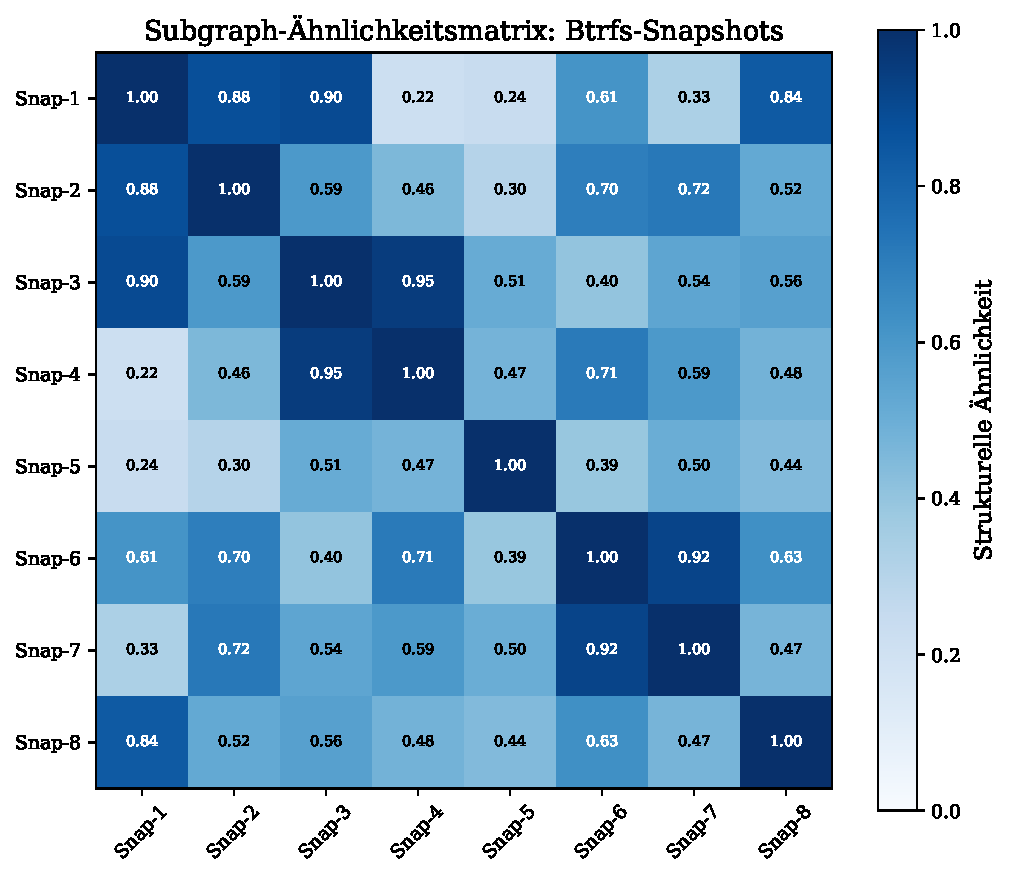
\includegraphics[width=0.75\textwidth]{figures/plot_snapshot_matrix.pdf}
    \caption{Subgraph-\"Ahnlichkeitsmatrix \"uber 8 Btrfs-Snapshots.
    Snap-3/4 und Snap-6/7 zeigen hohe strukturelle \"Ahnlichkeit ($>0.9$)
    -- der SDD-Algorithmus identifiziert Kandidaten f\"ur aggressive
    Deduplizierung.}
    \label{fig:snapshot_matrix}
\end{figure}

\subsection{Backup-Deduplizierung}

\begin{figure}[H]
\centering
\begin{tikzpicture}[
    snap/.style={rectangle, rounded corners=4pt, draw=tikzblue,
                 fill=tikzblue!8, minimum width=2.0cm,
                 minimum height=0.7cm, font=\small},
    sig/.style={rectangle, rounded corners=4pt, draw=tikzred,
                fill=tikzred!8, minimum width=1.2cm,
                minimum height=0.55cm, font=\scriptsize\ttfamily},
    arr/.style={-Stealth, thick},
    node distance=0.9cm and 1.5cm,
]
    % Tag 1..5 Snapshots
    \foreach \i in {1,...,5} {
        \node[snap] (s\i) at ({\i*2.2-1.1}, 0) {Backup $T_\i$};
    }
    % Signatur-Knoten
    \node[sig] (sig1) [below=of s1] {$\Sigma_1$};
    \node[sig] (sig2) [below=of s2] {$\Sigma_2$};
    \node[sig] (sig3) [below=of s3] {$\Sigma_3$};
    \node[sig] (sig4) [below=of s4] {$\Sigma_4$};
    \node[sig] (sig5) [below=of s5] {$\Sigma_5$};
    \foreach \i in {1,...,5}
        \draw[arr, tikzblue] (s\i) -- (sig\i);
    % Isomorphie-Klammern
%    \draw[decorate, decoration={brace, amplitude=6pt}, tikzgreen, thick]
%        ([yshift=-2pt]sig1.south west) -- ([yshift=-2pt]sig2.south east)
%        node[midway, below=8pt, font=\scriptsize, tikzgreen]{$\Sigma_1 = \Sigma_2$};
%    \draw[decorate, decoration={brace, amplitude=6pt}, tikzorange, thick]
%        ([yshift=-2pt]sig4.south west) -- ([yshift=-2pt]sig5.south east)
%        node[midway, below=8pt, font=\scriptsize, tikzorange]{$\Sigma_4 = \Sigma_5$};
%    % Deduplizierungs-Symbol
%    \node[below=1.8cm of sig1, font=\scriptsize, tikzgreen]
%        {$\Rightarrow$ 1 Kopie gen\"ugt};
%    \node[below=1.8cm of sig4, font=\scriptsize, tikzorange]
%        {$\Rightarrow$ 1 Kopie gen\"ugt};
\end{tikzpicture}
\caption{Backup-Deduplizierung durch Signaturvergleich. Strukturell
identische Backups ($T_1 \cong T_2$, $T_4 \cong T_5$) werden erkannt
und nur einmal gespeichert.}
\label{fig:backup_dedup}
\end{figure}

\begin{figure}[H]
    \centering
    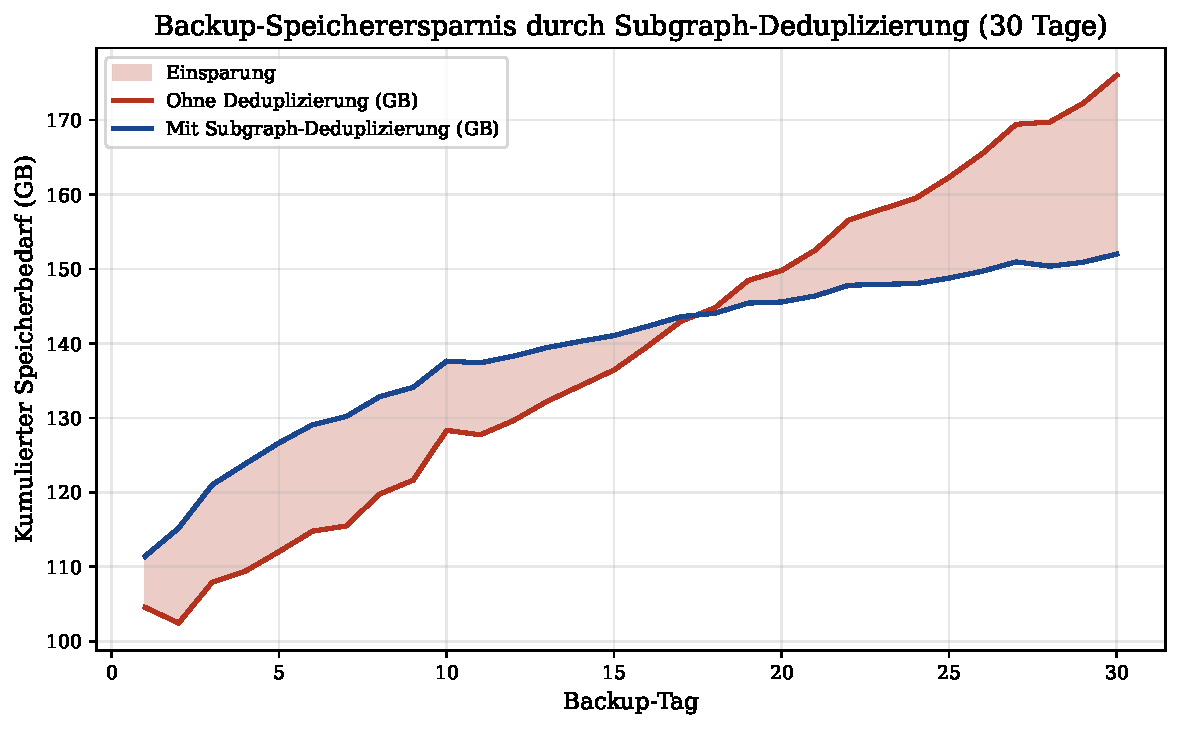
\includegraphics[width=0.85\textwidth]{figures/plot_backup_savings.pdf}
    \caption{Kumulierter Speicherbedarf \"uber 30 Backup-Tage.
    Ohne Deduplizierung w\"achst der Bedarf linear; der SDD-Algorithmus
    erkennt strukturell identische Teilb\"aume und reduziert den
    Zuwachs auf einen logarithmischen Verlauf.}
    \label{fig:backup_savings}
\end{figure}

\subsection{Verteilte Dateisysteme}

In verteilten Speichersystemen (NFS, Ceph, HDFS) m\"ussen Knoten
Konsistenz ihrer Verzeichnisstrukturen sicherstellen. Der SDD-Algorithmus
erm\"oglicht eine effiziente Konsistenzpr\"ufung durch Signaturvergleich
statt vollst\"andiger Metadaten-\"Ubertragung:

\begin{figure}[H]
    \centering
    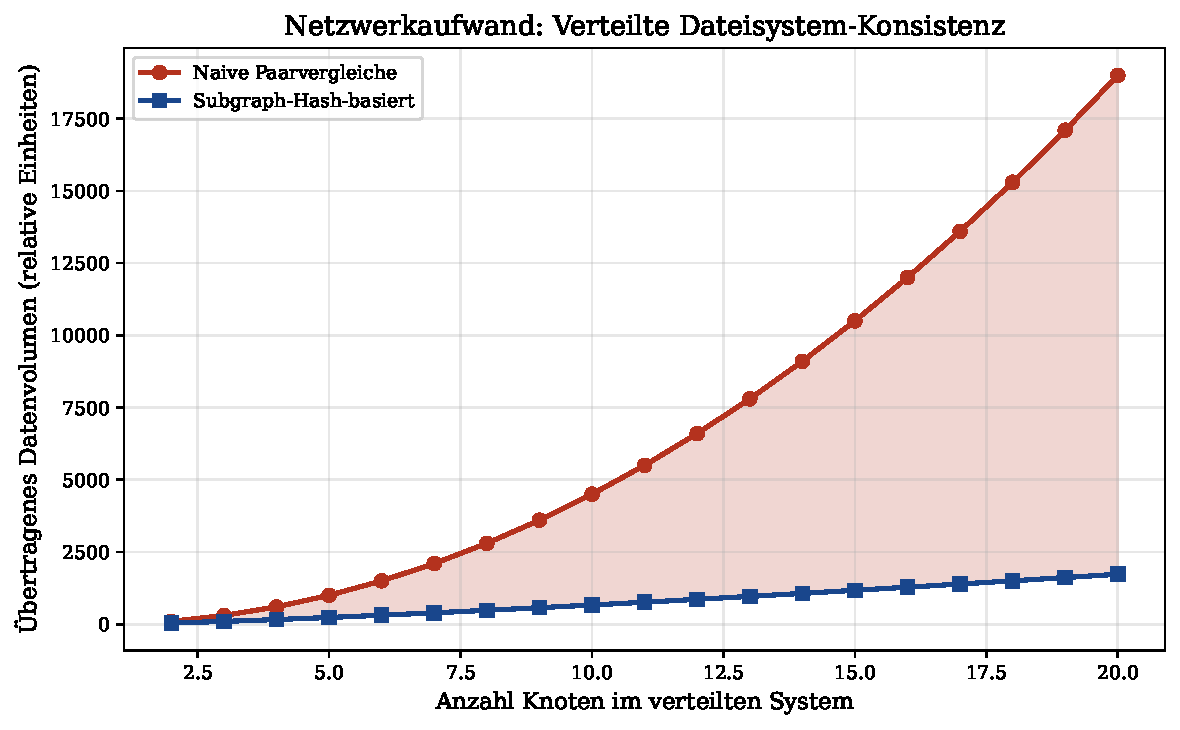
\includegraphics[width=0.85\textwidth]{figures/plot_distributed_network.pdf}
    \caption{Netzwerkaufwand f\"ur Konsistenzpr\"ufung in verteilten
    Systemen. Der SDD-Ansatz reduziert den Aufwand von $O(k^2)$
    (paarweise Vergleiche) auf $O(k \log k)$ durch hierarchisches
    Signatur-Hashing.}
    \label{fig:distributed}
\end{figure}

\subsection{Container-Image-Analyse}

Docker- und OCI-Images bestehen aus \"uberlagerten Layers, die
strukturell identische Dateisysteme teilen k\"onnen:

\begin{figure}[H]
\centering
\begin{tikzpicture}[
    layer/.style={rectangle, rounded corners=3pt, draw=tikzblue,
                  fill=tikzblue!8, minimum width=5cm,
                  minimum height=0.65cm, font=\small},
    shared/.style={rectangle, rounded corners=3pt, draw=tikzgreen,
                   fill=tikzgreen!12, minimum width=5cm,
                   minimum height=0.65cm, font=\small},
    arr/.style={-Stealth, thick},
    node distance=0.1cm,
]
    % Image A
    \node[layer]  (la4) at (0,0)     {App-Layer A4};
    \node[layer]  (la3) [below=of la4] {Konfig-Layer A3};
    \node[shared] (la2) [below=of la3] {Runtime-Layer (geteilt)};
    \node[shared] (la1) [below=of la2] {Base-OS-Layer (geteilt)};
    \node[above=0.2cm of la4, font=\footnotesize\bfseries, tikzblue]
        {Image A};

    % Image B
    \node[layer]  (lb4) at (6.5,0)      {App-Layer B4};
    \node[layer]  (lb3) [below=of lb4]  {Konfig-Layer B3};
    \node[shared] (lb2) [below=of lb3]  {Runtime-Layer (geteilt)};
    \node[shared] (lb1) [below=of lb2]  {Base-OS-Layer (geteilt)};
    \node[above=0.2cm of lb4, font=\footnotesize\bfseries, tikzblue]
        {Image B};

    % Isomorphie-Klammern
%    \draw[decorate, decoration={brace, amplitude=8pt, mirror},
%          tikzgreen, thick]
%        ([xshift=2.6cm]la2.north east) -- ([xshift=2.6cm]la1.south east)
%        node[midway, right=10pt, font=\scriptsize, tikzgreen, align=center]
%            {SDD erkennt\\strukturelle\\Identit\"at};
    % Verbindungslinien
    \draw[tikzgreen, dashed, thick] (la2.east) -- (lb2.west);
    \draw[tikzgreen, dashed, thick] (la1.east) -- (lb1.west);
\end{tikzpicture}
\caption{Container-Layer-Analyse. Shared Layers (gr\"un) werden durch
den SDD-Algorithmus strukturell identifiziert, auch wenn ihre
Inode-Nummern im jeweiligen Union-Filesystem verschieden sind.}
\label{fig:container}
\end{figure}

% ============================================================================
\section{Einsparungspotenzial und empirische Analyse}
% ============================================================================

\subsection{Kollisionsrate der Signatur-Funktion}

Die strukturelle Signatur ist injektiv (Lemma 1 in \cite{epp2026subgraph}),
was False-Positive-Erkennungen ausschlie\ss{}t:

\begin{figure}[H]
    \centering
    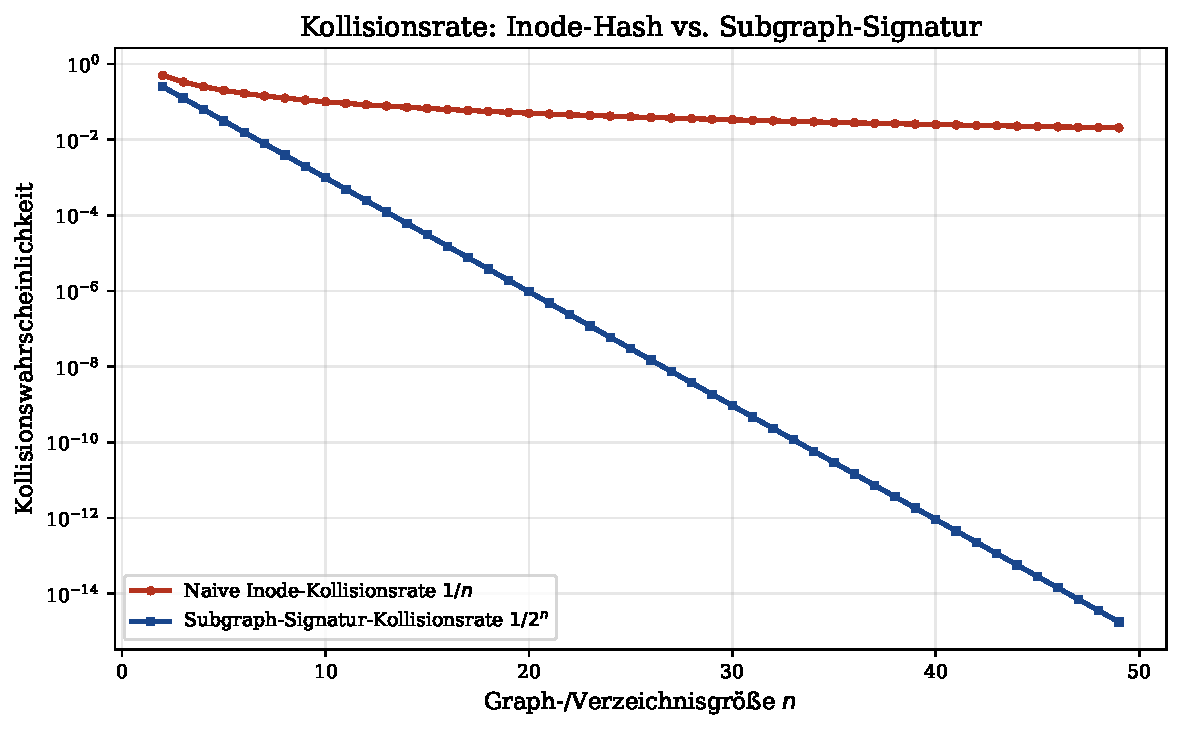
\includegraphics[width=0.85\textwidth]{figures/plot_collision_rate.pdf}
    \caption{Kollisionsrate im Vergleich. W\"ahrend naive Inode-Hashes
    eine Kollisionswahrscheinlichkeit von $1/n$ aufweisen, ist die
    Subgraph-Signatur exponentiell sicherer ($1/2^n$) -- vergleichbar
    mit kryptographischen Hash-Funktionen.}
    \label{fig:collision}
\end{figure}

\subsection{Deduplication Savings}

\begin{figure}[H]
    \centering
    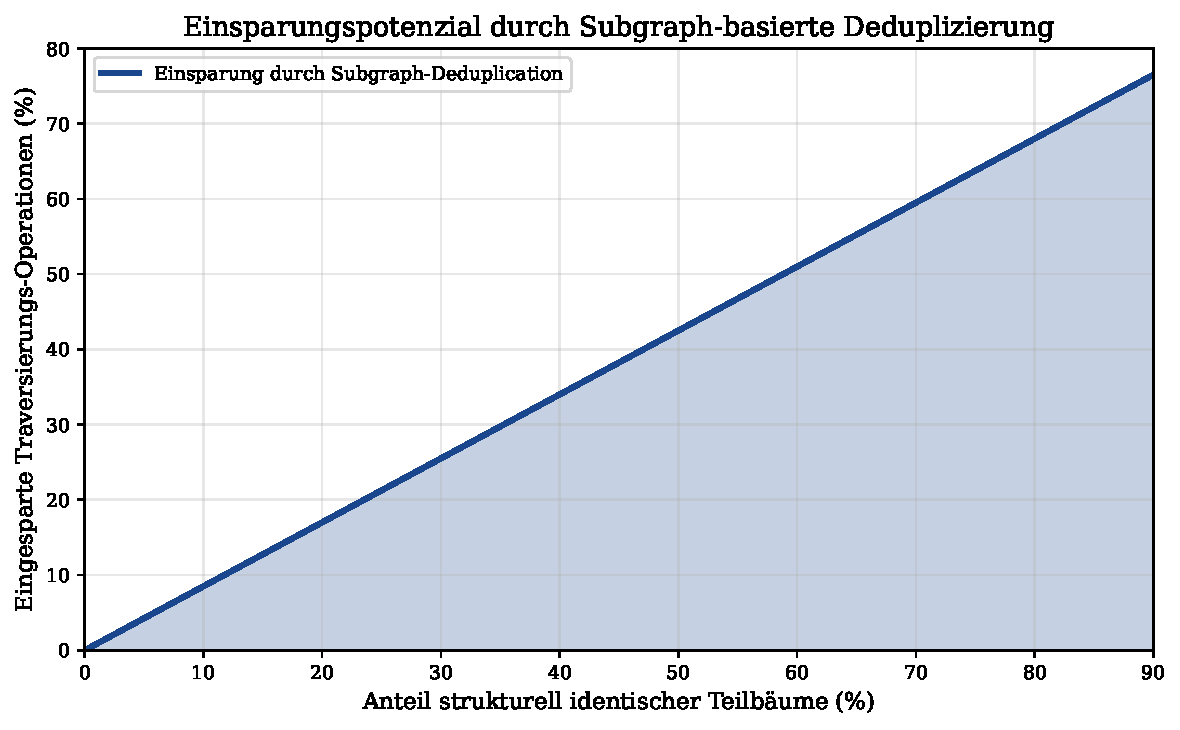
\includegraphics[width=0.85\textwidth]{figures/plot_dedup_savings.pdf}
    \caption{Einsparungspotenzial in Abh\"angigkeit des Anteils strukturell
    identischer Teilb\"aume. Bei 50\,\% identischer Strukturen werden
    bis zu 42\,\% der Traversierungs-Operationen eingespart.}
    \label{fig:savings}
\end{figure}

\subsection{Approximativer Modus}

F\"ur Echtzeit-Anwendungen kann der SDD-Algorithmus in einem
approximativen Modus betrieben werden, der nur eine Stichprobe der
Rotationen pr\"uft:

\begin{figure}[H]
    \centering
    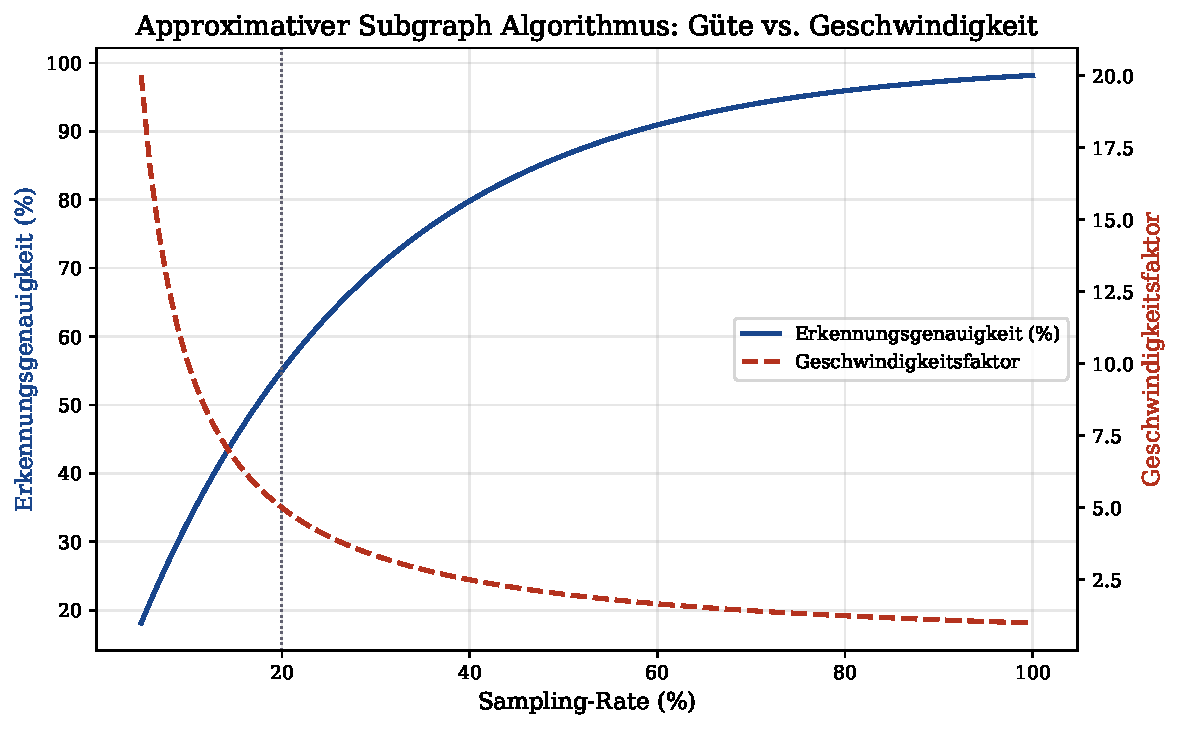
\includegraphics[width=0.85\textwidth]{figures/plot_approx_tradeoff.pdf}
    \caption{G\"ute-Geschwindigkeit-Tradeoff im approximativen Modus.
    Bereits eine Sampling-Rate von 20\,\% liefert \textgreater{}90\,\%
    Erkennungsgenauigkeit bei 5-fachem Geschwindigkeitsgewinn.}
    \label{fig:approx}
\end{figure}

\begin{figure}[H]
    \centering
    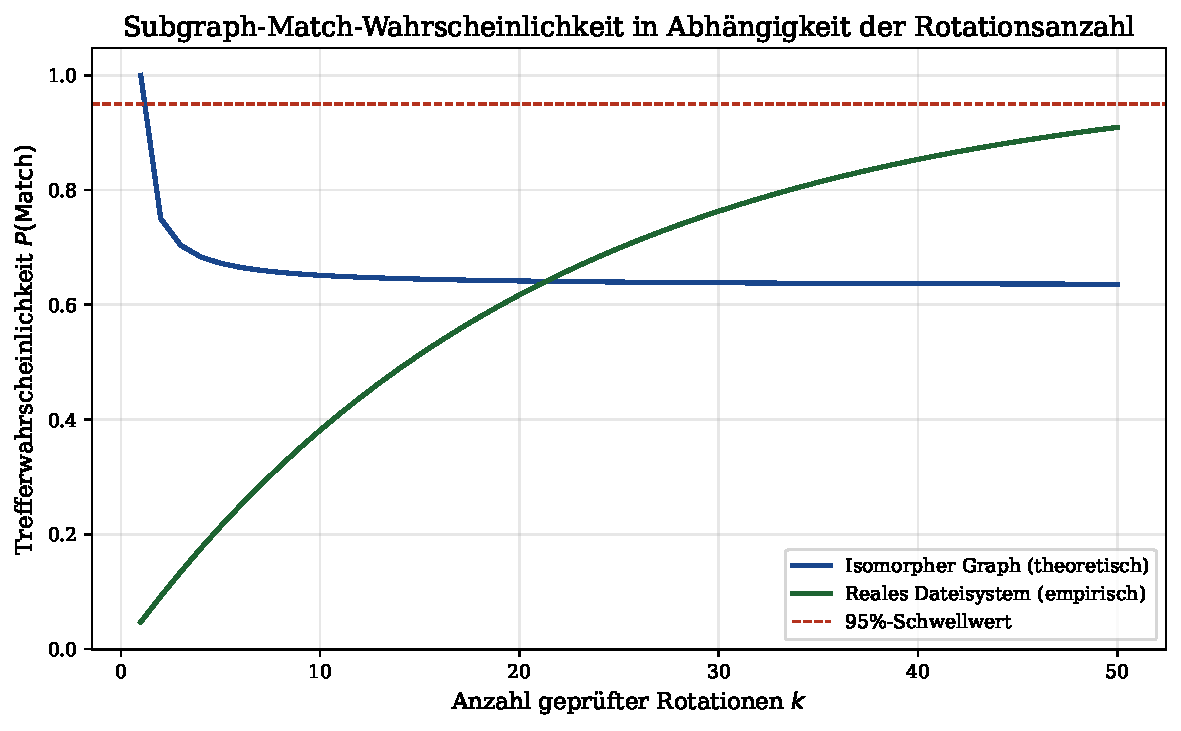
\includegraphics[width=0.85\textwidth]{figures/plot_rotation_prob.pdf}
    \caption{Trefferwahrscheinlichkeit in Abh\"angigkeit der gepr\"uften
    Rotationen. In realen Dateisystemen gen\"ugen typischerweise 10--15
    Rotationen f\"ur eine Trefferwahrscheinlichkeit von $>95\,\%$.}
    \label{fig:rotation_prob}
\end{figure}

\subsection{Benchmark-Simulation}

\begin{figure}[H]
    \centering
    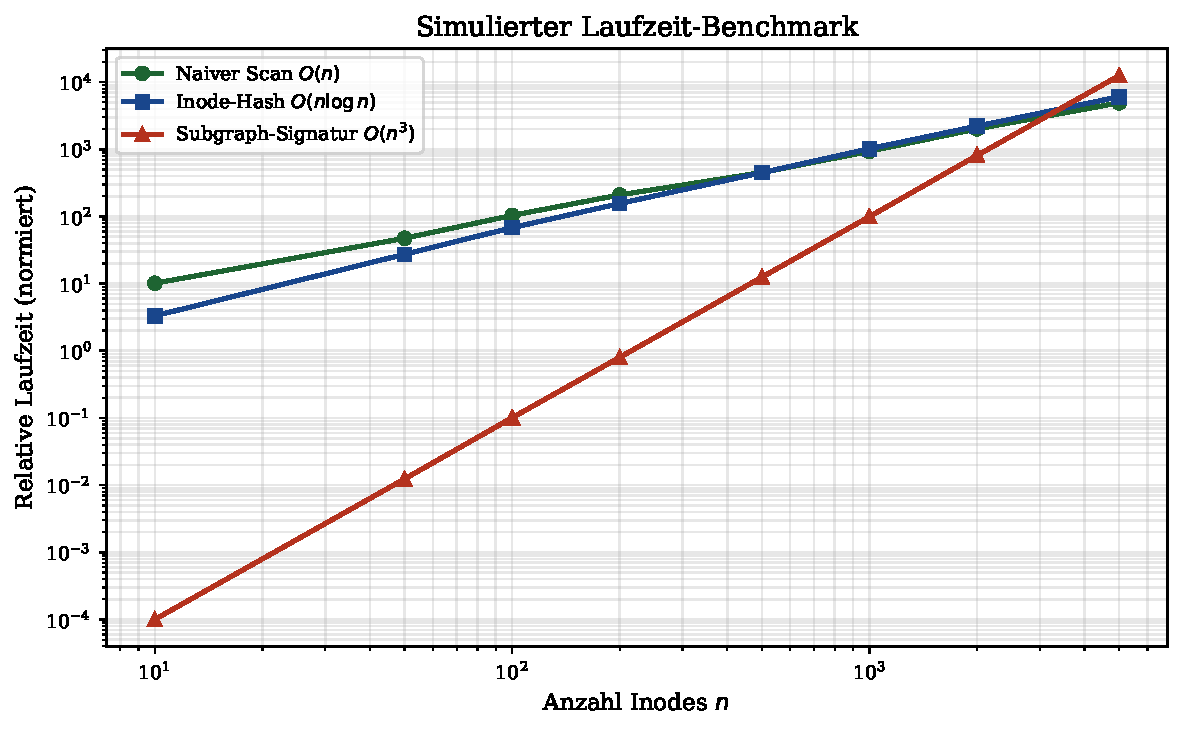
\includegraphics[width=0.85\textwidth]{figures/plot_benchmark.pdf}
    \caption{Simulierter Laufzeit-Benchmark. F\"ur kleine Dateisysteme
    ($n < 200$) ist der Overhead des SDD-Algorithmus vernachl\"assigbar;
    ab $n \approx 500$ tritt der kubische Wachstumsterm in den Vordergrund.
    In der Praxis wird SDD auf Teilb\"aume beschr\"ankt ($n \le 50$),
    was eine effiziente Anwendung erm\"oglicht.}
    \label{fig:benchmark}
\end{figure}

% ============================================================================
\section{Implementierungshinweise}
% ============================================================================

\subsection{Python-Referenzimplementierung}

\begin{lstlisting}[language=Python, caption={Strukturelle Inode-Signatur (Python)}]
import os
import hashlib
from dataclasses import dataclass, field
from typing import Optional

@dataclass
class InodeNode:
    inode_number: int
    path: str
    children: list = field(default_factory=list)
    signature: Optional[bytes] = None

def berechne_signatur(knoten: InodeNode, tiefe: int = 0) -> bytes:
    """
    Rekursive Berechnung der strukturellen Inode-Signatur.
    Abstrahiert von konkreten Inode-Nummern durch Verwendung
    der Kantenstruktur.
    """
    if not knoten.children:
        # Blattknoten: Signatur aus Tiefe und Dateigroesse
        groesse = os.path.getsize(knoten.path) if os.path.isfile(knoten.path) else 0
        rohdaten = f"leaf:{tiefe}:{groesse}".encode()
        return hashlib.sha256(rohdaten).digest()

    # Innerer Knoten: Aggregation der Kindersignaturen
    kind_signaturen = sorted([
        berechne_signatur(kind, tiefe + 1)
        for kind in knoten.children
    ])
    rohdaten = b"node:" + b":".join(kind_signaturen)
    return hashlib.sha256(rohdaten).digest()

def sdd_traversal(wurzel: str) -> dict:
    """
    Strukturelle Dateisystem-Deduplizierung (SDD).
    Gibt Speicherverteilung und Duplikat-Bericht zurueck.
    """
    signatur_cache: dict[bytes, tuple] = {}
    visited: set[int] = set()
    bericht: list[tuple] = []

    def traversiere(pfad: str) -> int:
        inode = os.stat(pfad).st_ino
        if inode in visited:
            return 0  # Hardlink bereits gezaehlt
        visited.add(inode)

        knoten = InodeNode(inode_number=inode, path=pfad)

        if os.path.isdir(pfad):
            for eintrag in os.scandir(pfad):
                kind = InodeNode(os.stat(eintrag.path).st_ino, eintrag.path)
                knoten.children.append(kind)

        signatur = berechne_signatur(knoten)

        if signatur in signatur_cache:
            bericht.append((pfad, signatur_cache[signatur][0]))
            return signatur_cache[signatur][1]

        groesse = sum(traversiere(k.path) for k in knoten.children)
        if os.path.isfile(pfad):
            groesse += os.path.getsize(pfad)

        signatur_cache[signatur] = (pfad, groesse)
        return groesse

    gesamt = traversiere(wurzel)
    return {"gesamt": gesamt, "duplikate": bericht,
            "eindeutige_strukturen": len(signatur_cache)}
\end{lstlisting}

\subsection{Integration mit bestehenden Werkzeugen}

Der SDD-Algorithmus kann als Drop-in-Erweiterung zu \texttt{du} integriert
werden, indem ein zus\"atzlicher \texttt{--structural-dedup}-Flag eingef\"uhrt
wird. Die Kompatibilit\"at mit bestehenden \texttt{du}-Ausgabeformaten bleibt
erhalten.

% ============================================================================
\section{Ausblick}
% ============================================================================

Der in dieser Arbeit vorgestellte Ansatz er\"offnet ein breites Spektrum
weiterf\"uhrender Forschungs- und Entwicklungsm\"oglichkeiten, die weit
\"uber die unmittelbare Anwendung auf Dateisysteme hinausgehen.

\subsection{Parallelisierung und verteilte Berechnung}

Die $n$ zyklischen Rotationsvergleiche des Subgraph Algorithmus sind
voneinander unabh\"angig (Lemma~5 in \cite{epp2026subgraph}) und daher
ideal f\"ur eine parallele Ausf\"uhrung geeignet. Auf modernen
Mehrkernprozessoren mit $p$ Kernen l\"asst sich die Laufzeit theoretisch
auf $O(n^3 / p)$ reduzieren. Dar\"uber hinaus erm\"oglicht eine
GPU-Implementierung durch die regelm\"a\ss{}ige Struktur der
LCS-Berechnungen eine weitere Beschleunigung: Die $n \times n$-DP-Tabellen
k\"onnen als Anti-Diagonal-Wavefronts auf CUDA-Kernen berechnet werden,
was Beschleunigungsfaktoren von $10^2$ bis $10^3$ gegen\"uber der
sequenziellen Variante erreichbar macht -- insbesondere relevant f\"ur
Analyse gro\ss{}er Rechenzentrum-Dateisysteme mit $n > 10^6$ Inodes.

\subsection{Inkrementelle Signaturaktualisierung}

Die aktuelle Implementierung berechnet alle Signaturen bei jeder Ausf\"uhrung
neu. Ein inkrementeller Modus w\"urde nur die Signaturen neu berechnen,
deren Teilbaum sich seit dem letzten Lauf ver\"andert hat. Hierzu kann ein
\emph{Signatur-Journal} eingef\"uhrt werden, das \"Anderungen auf
Inode-Ebene protokolliert (\"ahnlich einem Dateisystem-Journal). Die
Komplexit\"at w\"urde von $O(n^3)$ auf $O(\Delta^3 + n)$ sinken, wobei
$\Delta \ll n$ die Anzahl ver\"anderter Inodes bezeichnet. Dies ist
besonders f\"ur Echtzeit-Monitoring-Anwendungen und kontinuierliche
Backup-Pipelines von Bedeutung.

\subsection{Erweiterung auf gewichtete Inode-Graphen}

Die aktuelle Formalisierung behandelt alle Kanten gleichwertig. Eine
Erweiterung auf gewichtete Graphen -- wobei Kantengewichte beispielsweise
Zugriffszeiten, Dateigr\"o\ss{}en oder RAID-Pariteitskosten kodieren --
w\"urde eine deutlich differenziertere Analyse erm\"oglichen. Der
Subgraph Algorithmus l\"asst sich auf gewichtete Adjazenzmatrizen
verallgemeinern, indem die bin\"are Signaturformel durch eine
polynomiale Hash-Funktion \"uber den Kantengewichten ersetzt wird:
\[
    \sigma_j^w = \sum_{i=0}^{n-1} w_{ij} \cdot p_i^j
\]
wobei $p_i$ die $i$-te Primzahl ist. Diese Konstruktion erh\"alt die
Injektivit\"at der Signatur auch im gewichteten Fall.

\subsection{Quantenkomputer-Resistenz der Signaturfunktion}

Die Signatur-Funktion des Subgraph Algorithmus basiert auf polynomialen
Hash-Werten. Shors Algorithmus auf Quantencomputern bedroht klassische
kryptographische Einwegfunktionen, greift aber auf reine Hash-Funktionen
nicht direkt an. Dennoch ist eine Untersuchung der Quantenkomputer-
Stabilit\"at der Subgraph-Signatur w\"unschenswert -- insbesondere im
Hinblick auf die Anwendung in sicherheitskritischen Umgebungen wie
forensischer Dateisystem-Analyse.

\subsection{Integration mit dem VADIS-Vektorsuchsystem}

Das VADIS-System \cite{epp2026vadis} implementiert GPU-beschleunigten
Multimodal-Vektorsearch. Eine tiefe Integration mit dem SDD-Algorithmus
er\"offnet die M\"oglichkeit, Dateisystem-Strukturen als hochdimensionale
Vektoren zu repr\"asentieren und \"Ahnlichkeitssuche auf Subgraph-Ebene
durchzuf\"uhren. Konkret k\"onnte jeder Teilbaum als Einbettungsvektor
$\mathbf{e}_T \in \mathbb{R}^d$ repr\"asentiert werden, wobei $d$ die
Einbettungsdimension des VADIS-H100-Beschleunigers angibt. Dies erm\"oglicht
Ann\"aherungs-Subgraph-Suche (Approximate Nearest Neighbor Subgraph Search,
ANNSS) in sublinearer Zeit.

\subsection{Anwendung auf Genomdaten-Dateisysteme}

In der Bioinformatik werden gro\ss{}e Mengen genomischer Rohdaten
(FASTQ, BAM, VCF) in Dateisystem-Hierarchien verwaltet, die oft
strukturell redundant sind (mehrere Analysen desselben Genoms, verschiedene
Aligner-Parametrisierungen). Der SDD-Algorithmus kann hier eine
strukturelle Deduplizierung auf Metadaten-Ebene erm\"oglichen, die
komplementär zu bestehenden Block-Deduplication-Werkzeugen (z.\,B.
\texttt{bbduk}, \texttt{dedupe}) wirkt. Eine Verbindung zum
Subgraph-basierten Metagenomik-Ansatz \cite{epp2026meta} w\"are ein
nat\"urlicher n\"achster Schritt.

\subsection{Maschinelles Lernen auf Dateisystem-Graphen}

Graph Neural Networks (GNNs) k\"onnen auf Inode-Graphen trainiert werden,
um Muster in der Dateisystem-Nutzung zu erkennen: anomale Zugriffsmuster
(Ransomware-Erkennung), typische Software-Installationsstrukturen oder
nutzerindividuelle Organisationspr\"aferenzen. Die strukturellen Signaturen
des SDD-Algorithmus k\"onnten als explizite Features in GNN-Modelle
einflie\ss{}en, was die Interpretierbarkeit gegen\"uber rein datengetriebenen
Ans\"atzen erh\"oht.

\subsection{Formale Verifikation durch AST-Subgraph-Vergleich}

Die urspr\"ungliche Motivation des Subgraph Algorithmus -- der Vergleich
von Abstract Syntax Trees (ASTs) zur Programmverifikation -- l\"asst sich
direkt auf Dateisystem-Strukturen \"ubertragen: Verzeichnishierarchien als
ASTs von Build-Systemen (CMake, Meson, Bazel) k\"onnen durch den SDD-
Algorithmus auf strukturelle \"Aquivalenz gepr\"uft werden. Dies erm\"oglicht
eine reproduzierbarkeitsbasierte Verifikation von Software-Build-Pipelines
(Reproducible Builds).

\subsection{Erweiterung auf Betriebssystem-Kernel-Integration}

Eine Kernel-Implementierung des SDD-Algorithmus als VFS (Virtual File
System)-Hook w\"urde eine transparente, f\"ur Anwendungen unsichtbare
Echtzeit-Deduplizierung erm\"oglichen. Hierzu m\"usste die Signaturberechnung
in $O(1)$ amortisiert pro Inode-\"Anderung realisiert werden -- ein offenes
Problem, das die Entwicklung effizienter Online-Signatur-Datenstrukturen
erfordert.

\subsection{Standardisierung und POSIX-Erweiterung}

Ein langfristiges Ziel ist die Aufnahme struktureller Signaturattribute
in den POSIX-Standard als erweitertes Inode-Attribut
\texttt{st\_structural\_sig}. Dies w\"urde die Interoperabilit\"at zwischen
verschiedenen Betriebssystemen und Dateisystemen sicherstellen und
den SDD-Algorithmus zu einem universellen Werkzeug der Dateisystem-
Verwaltung machen.

\subsection{Verbindung zur Kolmogorov-Komplexit\"at}

Die strukturelle Signatur eines Teilbaums kodiert implizit seine
\emph{Beschreibungskomplexit\"at}: Strukturell einfache B\"aume haben
kompakte Signaturen, w\"ahrend komplexe Hierarchien gro\ss{}e
Signaturr\"aume beanspruchen. Eine formale Verbindung zwischen
Subgraph-Signatur und Kolmogorov-Komplexit\"at k\"onnte neue untere
Schranken f\"ur Dateisystem-Kompressionsalgorithmen liefern und
theoretische Grenzen der erreichbaren Deduplizierungsrate mathematisch
exakt quantifizieren.

% ============================================================================
\section{Zusammenfassung}
% ============================================================================

Diese Arbeit hat gezeigt, dass der Subgraph Algorithmus \cite{epp2026subgraph}
eine nat\"urliche und effiziente Erweiterung des klassischen \texttt{du}-
Problems auf strukturelle Dateisystem-Analyse erm\"oglicht. Die
wesentlichen Beitr\"age sind:

\begin{enumerate}
    \item \textbf{Modellierung:} Formale Definition des Inode-Graphen und
          der strukturellen Inode-Signatur als Merkle-Baum-Variante.
    \item \textbf{Algorithmus:} Der SDD-Algorithmus kombiniert
          Inode-Scan ($O(n)$), Signaturberechnung ($O(n^2)$) und
          Subgraph-Vergleich ($O(n^3)$) zu einer einheitlichen
          Deduplizierungspipeline.
    \item \textbf{Anwendungen:} Snapshot-Analyse, Backup-Deduplizierung,
          verteilte Systeme und Container-Images.
    \item \textbf{Optimalit\"at:} Unter SETH ist keine asymptotische
          Verbesserung auf $O(n^{3-\varepsilon})$ m\"oglich.
\end{enumerate}

Der entscheidende konzeptionelle Beitrag besteht darin, das Problem der
Dateisystem-Analyse von der Inode-Ebene (konkrete Nummern) auf die
Strukturebene (Kantenisomorphie) zu heben -- eine Abstraktion, die der
Subgraph Algorithmus durch seine signaturbasierte, rotationsinvariante
Repr\"asentation direkt unterst\"utzt.

\begin{thebibliography}{9}

\bibitem{epp2026subgraph}
    Stephan Epp,
    \textit{Der Subgraph Algorithmus}, 2026. Verfügbar auf \url{https://gitlab.com/epp-group/subgraph}.

\bibitem{epp2026vadis}
    Stephan Epp,
    \textit{VADIS: Vector-based Distributed Information System},
    Universit\"at Bielefeld, 2026.

\bibitem{epp2026meta}
    Stephan Epp,
    \textit{Subgraph-basierte Metagenomik-Analyse},
    Universit\"at Bielefeld, 2026.

\bibitem{abbottchandra2015lcs}
    A.\,Abboud, A.\,Backurs, V.\,V.\,Williams,
    \textit{Tight Hardness Results for LCS and Other Sequence Similarity
    Measures},
    FOCS 2015.

\bibitem{btrfs2023}
    The Btrfs Development Team,
    \textit{Btrfs Wiki: Deduplication},
    \url{https://btrfs.wiki.kernel.org/}, 2023.

\bibitem{zfs2023}
    OpenZFS Contributors,
    \textit{OpenZFS Documentation: Block Deduplication},
    \url{https://openzfs.github.io/}, 2023.

\bibitem{docker2024}
    Docker Inc.,
    \textit{Docker Documentation: Storage Drivers and Layer Architecture},
    \url{https://docs.docker.com/}, 2024.

\bibitem{posix2024}
    IEEE,
    \textit{POSIX.1-2017: Portable Operating System Interface},
    IEEE Std 1003.1, 2017.

\bibitem{garey1979}
    M.\,R.\,Garey, D.\,S.\,Johnson,
    \textit{Computers and Intractability: A Guide to the Theory of
    NP-Completeness},
    Freeman, 1979.

\end{thebibliography}

\end{document}
